\documentclass[a4paper,11pt]{article}
\usepackage[left=2.5cm, right=2.5cm, top=1.5cm, bottom=1.5cm]{geometry}
\usepackage{graphicx}
\usepackage{amssymb}
\usepackage{amsmath}
\usepackage{xcolor}
\usepackage[active,tightpage]{preview}
\usepackage{hyperref}
\usepackage{pythonhighlight}

\hypersetup{ %color attributes of citation, link, etc.
    colorlinks=true,
    linkcolor=blue,
    filecolor=gray,
    urlcolor=blue,
    citecolor=blue,
}

\setlength{\parindent}{0pt}

\renewcommand{\PreviewBorder}{1in}
\newcommand{\Newpage}{\end{preview}\begin{preview}}
\newcommand{\matlab}{\textsc{Matlab}} %very important and totally necessary addition
\newcommand{\parallelsum}{\mathbin{\!/\mkern-5mu/\!}}

\newcommand\Item[1][]{%
  \ifx\relax#1\relax  \item \else \item[#1] \fi
  \abovedisplayskip=0pt\abovedisplayshortskip=0pt~\vspace*{-\baselineskip}}

%'codify' text for snippets
\usepackage{xcolor}
\definecolor{codegray}{gray}{1}
\newcommand{\code}[1]{\colorbox{codegray}{\texttt{#1}}}


\graphicspath{ {../images/} }
           
\begin{document}
\begin{preview}
\title{\LARGE{\textbf{ECEN405 Lab 3 Report\\Asynchronous Buck Converter}}}
\author{Niels Clayton : 300437590\\\textbf{Lab Partner:} Nickolai Wolfe}
\date{}
\maketitle
\hrule

\section{MOSFET Source Voltage}
  
  \begin{center}
    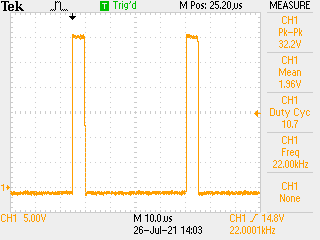
\includegraphics[width=0.8\textwidth]{continuious_opperation.png}

    \textit{High side MOSFET source voltage at 10\% duty cycle}
  \end{center}

  The waveform shown above is from the source of the high-side MOSFET. This signal looks mostly the same as the PWM control signal into the gate driver, with a 10\% duty cycle, and a 22kHz frequency. The major difference however, is that it now has a peak to peak voltage of 30V, as that is the supply into the drain of the high side MOSFET.
  

\section{Efficiency vs Output Current Plot} 

  \begin{center}
    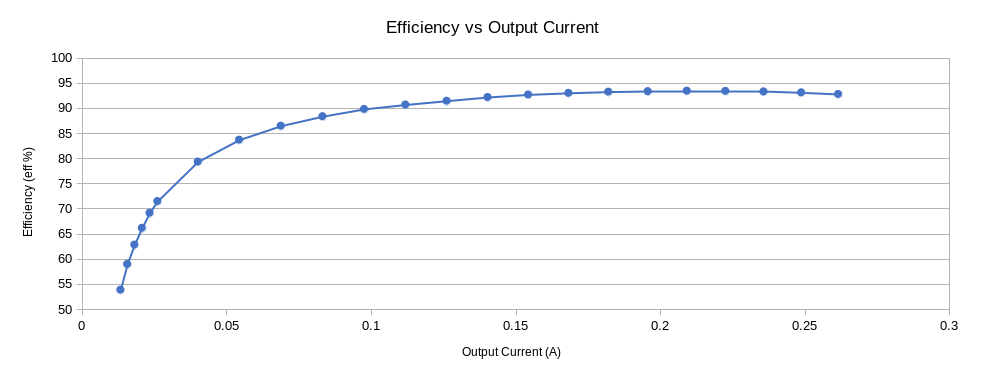
\includegraphics[width=\textwidth]{sync_buck.png}

    \textit{Efficiency vs output current plot for a non-synchronous buck converter}
  \end{center}

  From the efficiency vs output current plot above, we can clearly see that as the output current increases the overall efficiency of the converter increases, tapering off at 90\% at 150mA. The conduction losses in this system are dependant on the duty cycle of the of the PWM control signal, increasing and decreasing with this duty cycle due to the changing conduction period. The switching losses within the system will remain constant assuming a constant load, since the switching frequency has not changed. From this we know that at low current output the majority of the losses will be due to the switching losses. As the output current increases the conduction losses will will represent a larger portion of the losses. 
 
\section{Synchronous vs Non-Synchronous Efficiency}
  

  \begin{center}
    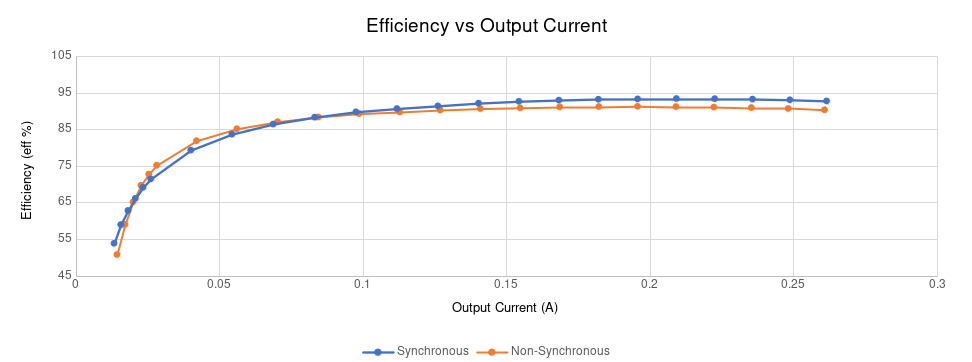
\includegraphics[width=\textwidth]{sync_vs_non-sync.png}
  \end{center}

  In the plot above we can see the comparison between the efficiency curves of the synchronous and no-synchronous buck converter topologies. From this plot we can see that for our 100$\Omega$ load they have very similar efficiency vs output curves. It can however be seen that at higher output currents the synchronous topology has a slightly higher efficiency. This is due to the losses created by the diode drop of the non-synchronous topology, since this diode drop is constant, at high output currents there will be large losses across the diode. 


\section{Application and Usage}

The non-synchronous buck converter topology offers a simpler to implement and often lower cost design compared to the synchronous. This is due to the replacement of a MOSFET with a power diode that is often cheaper to purchase, and the use of a more simple MOSFET gate driver. Because of this, the non-synchronous topology is often used when cost is a driving factor, and efficiency is not required. Due to its simpler design, the non-synchronous topology is also easier to build quickly on a breadboard when a voltage step-down is required. 

\section{Reduced Switching Frequency (Discontinuous Conduction)}
  
  \begin{center}
    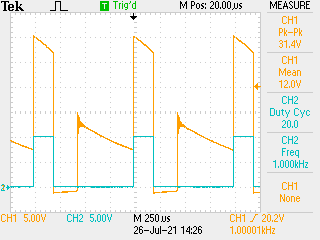
\includegraphics[width=0.8\textwidth]{discontinuious_opperation.png}
  \end{center}



\end{preview}
\end{document}